\chapter{2022}

\section*{一、 选择题 (本大题共 15 小题, 每小题 2 分, 共 30 分)}

1. 当输入非法错误时,一个“好”的算法会进行适当处理,而不会产生难以理解的输出结果。 这称为算法的(   )。

A. 可读性 B. 健壮性 C. 正确性 D. 有穷性

2. 当字符序列 F4\_作为一个栈的输入时,输出长度为 3 的且可用作 C 语言标识符的序列有(   )个。

A. 4 B. 5 C. 3 D. 6

3. 若用一个大小为 7 的数组来实现循环队列, 且当前 rear 和 front 的值分别为 0 和 4 , 当从队列中删除一个元素,再加入两个元素后, rear 和 front 的值分别为(   )。

A. 2 和 6 B. 6 和 2 C. 5 和 2 D. 2 和 5

4. 用一个栈求下列后缀表达式的值,
\begin{center}
    \verb|8 2 3 ^ / 2 3 * + 5 1 * -|
\end{center}

其中:+、-、*、/、\^分别是加、减、乘、除、幂运算符,当扫描到第一个*时,栈顶部 2 个元素是(   )。

A.6,1 B.5,7 C.3,2 D.1,5

5. 某二叉树的前序序列和后序序列正好相反,则该二叉树一定是(   )的二叉树。

A. 空或只有一个节点 B. 高度等于其节点数

C. 任一节点无左孩子 D. 任一节点无右孩子

6. 一棵左子树为空的二叉树在前序线索化后,其中空的链域的个数是(   )。

A. 不确定 B. 0 C. 1 D. 2

7. (   ) 占用的额外空间的空间复杂性为 \(O\left( 1\right)\) 。

A. 堆排序算法 B. 归并排序算法

C. 快速排序算法 D. 以上答案都不对

8. 在 Huffman 编码中, 若编码长度只允许小于等于 3 , 则除了已对两个字符编码为 0 和 10 外,还可以最多对(   )个字符编码。

A. 2 B. 3 C. 4 D. 5

9. 设一个稀疏矩阵有 1000 行 850 列, 其中有 800 个非 0 元素。设每个整数占 \(2\mathrm{\;B}\) , 数据值占 4B,则用三元组表存储该矩阵时所需字节数是(   )。

A. 1600 B. 3200 C. 6400 D. 9600

10. 用于求无向图的所有连通分量的算法是(   )。

A. 广度优先遍历 B. 拓扑排序 C. 求最短路径 D. 求关键路径

11. 若需在 \(O\left( {n{\log }_{2}n}\right)\) 的时间内完成对数组的排序,且要求排序是稳定的,则可选择的排序方法是(   )。

A. 快速排序 B. 堆排序 C. 归并排序 D. 直接插入排序

12. 下列(   )的邻接矩阵是对称矩阵。

A. AOV 网 B. AOE 网 C. 有向图 D. 无向图

13. 将元素 71、65、84、69、67、83 逐个插入空的二叉排序树(BST)中,最低层的元素为 (   )。

A. 65 B. 67 C. 69 D. 83

14. 具有 12 个关键字的有序表,折半查找的平均查找长度为(   )。

A. 3.1 B. 4 C. 2.5 D. 5

15. 若在一棵 \(m\) 阶 \(\mathrm{B}\) 树的结点中插入新关键码后该结点必须分裂为两个结点,那么在插入前结点的关键码数应为(   )。

A. \(m\) B. \(m - 1\) C. \(m + 1\) D. \(m - 2\)

\section*{二、填空题(本大题共 10 小题,每小题 3 分,共 30 分)}

16. 对于具有 144 个记录的文件, 若采用分块查找法, 且每块长度为 8 , 采用顺序查找确定所在的块,则平均查找长度为(   )。

17. A、B、C、D、E、F和G这七个元素以相反的顺序被压入堆栈，即从G开始。堆栈被弹出五次，每个元素被插入到队列中。从队列中删除两个元素并将其推回到堆栈中。现在，一个元素被弹出从堆栈中。弹出的项是(   ).

18. 有 \(n\) 个字符的字符串的非空子串个数最多有(   )个。

19. 用有向无环图描述表达式 \({\left( a + b\right) }^{ * }\left( {\left( {a + b}\right) /a}\right)\) ,至少需要顶点的数目为(   )。

20. 由 3 个结点可以构造出(   )种不同的二叉树。

21. 若一个具有 \(n\) 个顶点, \(e\) 条边的无向图是一个森林,则该森林中必有(   )棵树。

22. 对于长度为 18 的有序顺序表, 若采用折半查找, 则查找第 15 个元素的查找次数为 (   )。

23. (   )是哈希表的一个重要参数,它反映哈希表的装 满程度。

24. 硬件厂商 XYZ 公司宣称他们最新研制的微处理器运行速度为其竞争对手 ABC 公司同类产品的 100 倍。对于计算复杂度为 \({n}^{2}\) 的算法,若用 \(\mathrm{{ABC}}\) 公司的计算机能在 1 小时内解输入规模为 \(n\) 的问题,那么用 XYZ 公司的计算机在 1 小时内能解输入规模为 (   ) 的问题。

25. 表达式 \(A/B + D\$ E + F/H\) 中,运算符的优先级由高到低依次为 \(+ ,/,\$\) ,均右结合,则相应的后缀式是 (   )。

\section*{三、 综合应用题 (本大题共 7 小题, 共 60 分)}

26. (5 分) 阅读代码, 函数 print(   )接收 二叉查找树/二叉排序树(BST)的根和 一个正整数 \(k\) 作为参数。请:

// a BST node
\begin{lstlisting}[language=C, basicstyle=\ttfamily]
struct node { 
    int data;
    struct node *left, *right;
};
int count = 0;
void print(struct node *root, int k)
{
    if(root != NULL&&count<=k)
    {
        print(root->right, k);
        count++;
        if(count==k)
            printf("%d", root->data);
        print(root->left, k);
    }
}
\end{lstlisting}

(1)简述该代码的功能；

(2)print(root, 3)的输出是什么?其中 root 表示下图 BST 树的根。

\begin{center}
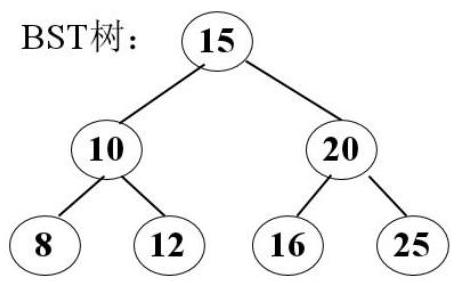
\includegraphics[width=0.3\textwidth]{images/2022/comprehensive_26.jpg}
\end{center}
\vspace{10em}

27. (5 分) 有一段代码:
\begin{lstlisting}[language=C, basicstyle=\ttfamily]
int count = 0;
for (int i=0;i<N;++)
    for (int j=i+1;j<N;j++)
        for (int k=j+1;k<N;k++)
            if (a[i]+a[j]>=a[k])count++;
\end{lstlisting}

假设 \(\mathrm{N} = {1000}\) 时,执行这段代码需要 1 秒时间。现在对这段代码的运行时间 (秒) 进行预估,请用一个关于 \(N\) 的函数来表示。
\vspace{10em}

\newpage
28. (10分)设 \(\mathrm{A},\mathrm{B},\mathrm{C},\mathrm{D},\mathrm{E}\) 五个字符的编码分别为1,2,3,4,5,并设标识符按以下次序出现: AA, BB, BD, BE, AB, AD, CD, BC, AE, DD。要求用哈希 (Hash) 方法将它们存入具有 10 个位置的表中。

(1)将上述关键字(标识符)构造一个哈希函数, 使得发生冲突尽可能地少;

(2)采用线性探测再散列法解决冲突, 写出上述各关键字在表中的位置, 并给出比较次数；即:填写完整下表。
\begin{center}
\begin{tabular}{|c|c|c|c|c|c|c|c|c|c|c|}
\hline
哈希地址 & 0 & 1 & 2 & 3 & 4 & 5 & 6 & 7 & 8 & 9 \\
\cline{1-11}
关键字 & \phantom{X} & \phantom{X} & \phantom{X} & \phantom{X} & \phantom{X} & \phantom{X} & \phantom{X} & \phantom{X} & \phantom{X} & \phantom{X} \\
\cline{1-11}
比较次数 & \phantom{X} & \phantom{X} & \phantom{X} & \phantom{X} & \phantom{X} & \phantom{X} & \phantom{X} & \phantom{X} & \phantom{X} & \phantom{X} \\
\cline{1-11}
\hline
\end{tabular}
\end{center}
\vspace{15em}

29. (10分)已知一棵二叉查找树/二叉排序树(BST)的先序遍历序列为30,20,10,15, 25,23,39,35,42。

(1)请画出此二叉树的形态。

(2)请给出这棵树的后序遍历序列。

(3)画出此二叉树的中序线索二叉树。

(4)画出与此二叉树对应的森林。
\vspace{10em}

\newpage
30. (12 分) 已知图 \(G\) 如右边所示:

\begin{figure}[htbp]
    \centering
    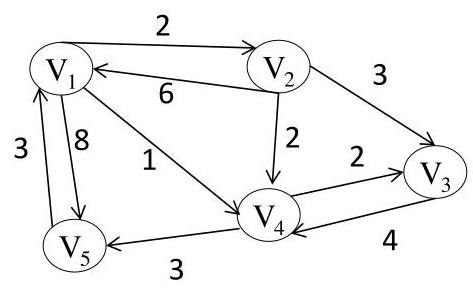
\includegraphics[width=0.3\textwidth]{images/2022/comprehensive_30.jpg}
    \caption*{图G} % 使用带星号的 caption*
\end{figure}
(1)画出 \(G\) 的邻接表表示图；

(2)根据你画的邻接表,以顶点 \({V}_{1}\) 为根,画出 \(G\) 的深度优先生成树;

(3)利用弗洛伊德算法(Floyd)求每一对顶点之间的最短路径, 请给出带权长度矩阵

\({\mathbf{D}}^{\left( 0\right) },{\mathbf{D}}^{\left( 1\right) }\) 和 \({\mathbf{D}}^{\left( 2\right) }\) 。
\vspace{10em}

31. (8分)考虑序列:‘mississippi’,请:

(1)采用赫夫曼(Huffman)编码算法对上述序列编码, 给出相应的 Huffman 树, 以及每个字符的 Huffman 码。 

(2)一共需要多少 bit 位?
\vspace{10em}

\newpage
32. (10 分)下表 32-1 中第 0 行是待排序序列的原始输入(Eagle Ant Dog Frog Cat Horse Bee Goat); 其他各行是 5 种排序算法得到的某个中间步骤的内容。 表 32-2 列出了 6 种排序算法。

请按行序直接给出每行对应排序算法的编号。每个编号只使用一次。

表 32-1: 行号 排序算法 序列

\begin{table}[htbp]
\centering
\caption{表 32-1}
\begin{tabular}{lll}
\toprule
行号 & 排序算法 & 序列 \\
\midrule
\textbf{第0行} & \textbf{原始输入} & \textbf{Eagle Ant Dog Frog Cat Horse Bee Goat} \\
\midrule
& 算法 1: & Ant Dog Eagle Frog Cat Horse Bee Goat \\
& 算法 2: & Ant Dog Eagle Frog Bee Cat Goat Horse \\
& 算法 3: & Ant Bee Dog Frog Cat Horse Eagle Goat \\
& 算法 4: & Bee Ant Dog Eagle Cat Horse Frog Goat \\
& 算法 5: & Bee Ant Dog Cat Eagle Horse Frog Goat \\
\bottomrule
\end{tabular}
\end{table}

\begin{center}
\begin{tabular}{|c|c|c|c|c|c|c|c|c|c|}
\hline
算法 3: & \phantom{X} & Ant & Bee & Dog & Frog & Cat & Horse & Eagle & Goat \\
\cline{1-10}
算法 4: & \phantom{X} & Bee & Ant & Dog & Eagle & Cat & Horse & Frog & Goat \\
\cline{1-10}
算法 5: & \phantom{X} & Bee & Ant & Dog & Cat & Eagle & Horse & Frog & Goat \\
\cline{1-10}
\hline
\end{tabular}
\end{center}

表 32-2:

\begin{center}
\begin{tabular}{|c|c|}
\hline
排序算法编号 & 排序算法名称 \\
\cline{1-2}
A & 冒泡排序 \\
\cline{1-2}
B & 直接插入排序 \\
\cline{1-2}
C & 希尔排序(增量为 3, 1) \\
\cline{1-2}
D & 快速排序 \\
\cline{1-2}
E & 简单选择排序 \\
\cline{1-2}
F & 二路归并排序 \\
\cline{1-2}
\hline
\end{tabular}

\end{center}
\vspace{20em}

\section*{四、算法分析与设计题 (本大题共 2 小题, 共 30 分)}

33. (15 分)设计一个算法,将一个用循环链表表示的稀疏多项式分解成两个多项式,使这两个多项式中各自仅含奇次项或偶次项, 并要求利用原链表中的结点空间构成这两个链表。要求:

(1)描述算法的基本设计思想；

(2)根据设计思想,采用 \(\mathrm{C}\) 或 \(\mathrm{C} +  +\) 语言描述算法,关键之处给出注释；

(3)说明所设计算法的时间复杂度和空间复杂度。
\vspace{6em}

提示: 其中稀疏多项式采用的循环链表存储结构 LinkedPoly 定义为
\begin{lstlisting}[language=C, basicstyle=\ttfamily]
typedef struct PolyNode {
    float coef; //单项式的系数
    int exp; //单项式的指数
    struct PolyNode *next;
}PolyNode;
typedef PolyNode*LinkedPoly;
\end{lstlisting}

算法描述,只需要给出如何将循环链表 \(\mathrm{L}\) 分成满足要求的两个循环链表的操作,即完善下述函数: 
\begin{lstlisting}[language=C, basicstyle=\ttfamily]
void Divide (LinkedPoly L) {
......
}
\end{lstlisting}
\vspace{20em}


34. (15分) 从根到叶子的最大距离称为树的半径。给定一个无向连通图,写一个算法找出半径最小的生成树。要求:

(1)描述算法的基本设计思想；

(2)根据设计思想,采用 \(\mathrm{C}\) 或 \(\mathrm{C} +  +\) 语言描述算法,关键之处给出注释；

(3)说明所设计算法的时间复杂度和空间复杂度。